\section{Project Goal and Approach}

\textit{Space Oddities} turns satellite catalogue data into a story that anyone can follow.
The raw data (SATCAT catalogues, Two-Line Element sets, Conjunction Data Messages) is used daily by space agencies but is completely unreadable to a general audience.

The format is scrollytelling, inspired by \href{https://pudding.cool/2017/10/satellites/}{The Pudding}.
In chapters 1 to 3, a single orbital map is pinned on the left while chapter cards scroll on the right, each filtering, recolouring, or labelling the same scene.
In chapters 4 to 6, the left panel becomes domain-specific controls (a collision event list, then a CDM table) while the charts scroll alongside.

\section{Chapters and Key Visualizations}

\subsection{Chapter 1: The Exponential Growth}
\textit{Story:} The space around Earth was once sparse, but has rapidly filled up, especially after 2019.

\textit{Visualization:} A 2D Canvas orbital scene shows around 68\,000 objects in orbit. Positions are computed from the latest available TLE using the SGP4 model via \texttt{satellite.js}, updated every 2 seconds to show continuous motion, with deorbited objects filtered out. A scroll-linked year slider progressively fills the map from 1957 to today. A D3 area/line chart shows yearly launches and the running total.

\subsection{Chapter 2: Where Do They Orbit?}
\textit{Story:} Satellites are not randomly distributed, but organized into distinct orbital regions dominated by different uses and actors. LEO is the most crowded region.

\textit{Visualization:} The same orbital scene is recoloured by orbit band (LEO/MEO/GEO). A D3 bar chart shows object counts per band, and hovering a bar highlights only the corresponding satellites in the map.

\subsection{Chapter 3: Payloads vs.\ Debris}
\textit{Story:} A large share of what orbits Earth is no longer active satellites, but debris.

\textit{Visualization:} The orbital scene remains the main view, with type filter buttons to hide or show object categories. A D3 donut chart shows the payload/debris/rocket-body split, while selecting a category updates the map accordingly.

\subsection{Chapter 4: Kessler Syndrome}
\textit{Story:} In orbit, one collision can create debris that increases the probability of future collisions.

\textit{Visualization:} A list of real historical events is linked to the map, with hover-to-zoom on the corresponding case. A D3 debris-count line chart shows the evolution of fragmentation, with a filter on minimum object size ($>$\,1\,mm to $>$\,1\,m).

\subsection{Chapter 5: Visualizing the Invisible Risk}
\textit{Story:} Collision risk is hard to grasp because near misses happen at extreme speed and usually remain invisible in raw tables.

\textit{Visualization:} A filterable and sortable sticky CDM table lists 3\,761 conjunction events. Picking a row reveals two satellite info cards, a 2D orbit-pair canvas, a time slider, and a D3 approach-distance graph. This turns abstract CDM values into a concrete close-approach visualization.

\subsection{Chapter 6: The Margin of Error}
\textit{Story:} Satellite trajectories are uncertain, and this uncertainty is part of what makes close approaches dangerous.

\textit{Visualization:} The CDM table remains fixed while the selected event is explored further. At TCA, 2D covariance ellipses are drawn around the two objects, the overlap region is shaded, and $P_c$ is labelled. This makes the margin of error visible instead of an abstract probability.

\subsection*{Extra Features}
These features are optional additions on top of the MVP and will be implemented if time allows.
\begin{itemize}[noitemsep, topsep=3pt]
    \item \textbf{Kessler Cascade Simulator (Ch.\ 4):} Canvas animation of a ring of orbiting objects where a triggered collision causes fragments to spread and hit other objects.
    \item \textbf{Car Highway Comparison (Ch.\ 5):} SVG of two cars on a road with the gap scaled to the selected CDM miss distance and a time-to-contact label at orbital speed (~7\,km/s).
    \item \textbf{3D Margin of Error (Ch.\ 6):} Three.js view of uncertainty ellipsoids around TCA, rotatable by the user.
\end{itemize}

\section{Data, Tools and Lectures}

\textbf{Data:}
Space-Track.org SATCAT and TLE (around 68\,000 objects); UCS Satellite Database (operator and owner metadata, joined on NORAD ID); 3\,761 emergency-reportable CDMs covering 1\,046 unique satellite pairs.

\textbf{Tools:}
\begin{itemize}[noitemsep, topsep=3pt]
    \item \textbf{React + Vite:} Component-based frontend; each chapter, sticky panel, CDM table, and satellite cards are separate components.
    \item \textbf{D3.js:} All statistical charts (area, bar, donut, line) and canvas quadtree hit-testing.
    \item \textbf{Canvas 2D API:} Orbital scene, orbit pair canvas, covariance ellipses, and the Kessler simulator (extra).
    \item \textbf{satellite.js (SGP4):} In-browser propagation; the approach distance graph computes positions at 2-minute intervals on demand.
    \item \textbf{Three.js / WebGL:} 3D covariance view (extra feature, Ch.\ 6).
    \item \textbf{Mantine:} UI primitives (badges, dividers).
    \item \textbf{Python (pandas, numpy):} Offline merge of SATCAT, UCS, and TLE files into \texttt{objects.csv}, \texttt{tle.csv}, \texttt{conjunction\_events.csv}.
\end{itemize}

\textbf{Relevant COM-480 Lectures:}
\begin{itemize}[noitemsep, topsep=3pt]
    \item \textbf{Storytelling:} To structure the project as a "scrollytelling" experience with clear chapters and a guided narrative, as the website user is scrolling down, the different chapters unravel in a linear way.
    
    \item \textbf{Interaction, Views:} For scroll-linked transitions, filtering, and linked views between the orbital map, charts, and tables. For example, in Chapter 2, hovering a bar in the orbit distribution chart highlights only the corresponding satellites in the orbital map)
    
    \item \textbf{Perception, Color:} To help design readable color schemes and manage visual attention in a very dense scene, as the orbital map has thousands of objects. It should be easy to distinguish categories, for example in Chapter 2 where orbit types (LEO, MEO, GEO) are encoded with clearly separated colors.
    
    \item \textbf{Tabular Data:} To get inspiration on how to represent data effectively through charts (line, bar, donut) linked to the orbital map. For example, in Chapter 1, the yearly launches are summarized in a line/area chart.
    
    \item \textbf{D3.js:} Used to build charts and handle interactions between views (e.g. updating the bar chart and highlighting the corresponding satellites on the map on hover).
    
    \item \textbf{JavaScript, DOM:} To manage the page structure and interactions (scroll events, dynamic updates, data loading), especially for linking the scrollytelling flow with the different visual components.
\end{itemize}

\section{Website Link}
\href{https://com-480-data-visualization.github.io/space-oddities/}{Website link}

\begin{figure}[H]
    \centering
    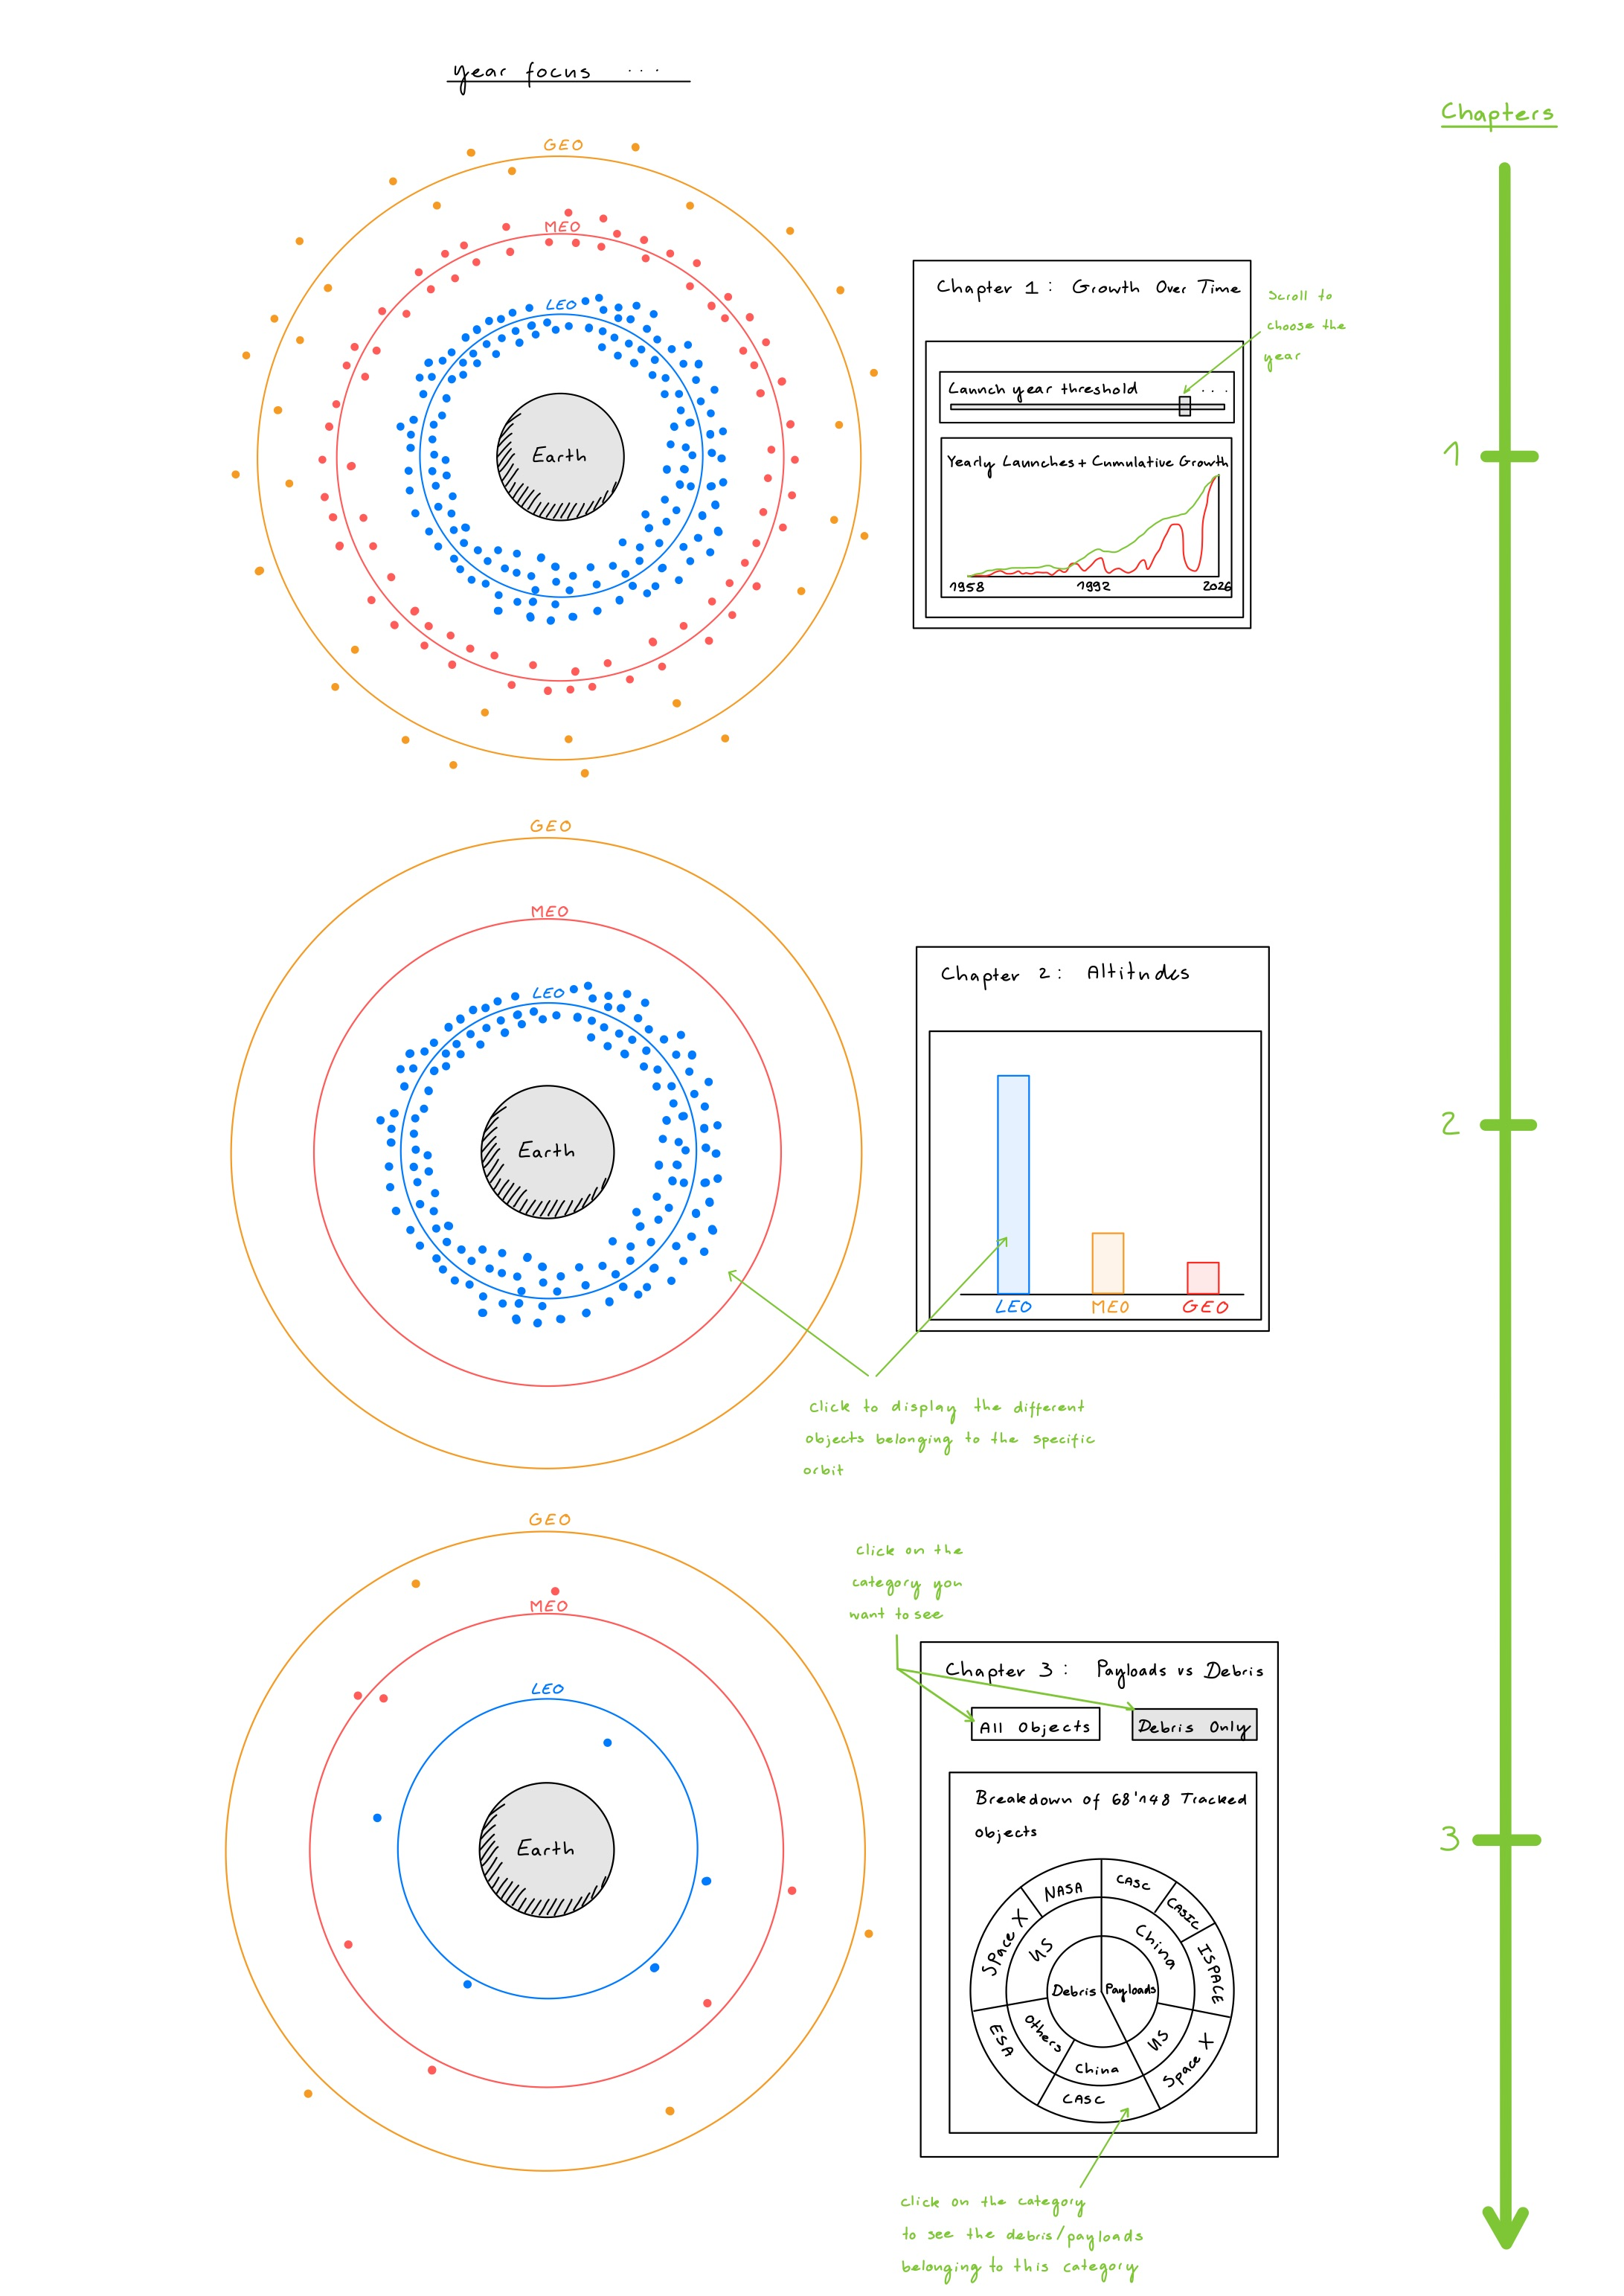
\includegraphics[width=1\linewidth]{Data Vizualization-8 2.jpg}
\end{figure}

\begin{figure}[H]
    \centering
    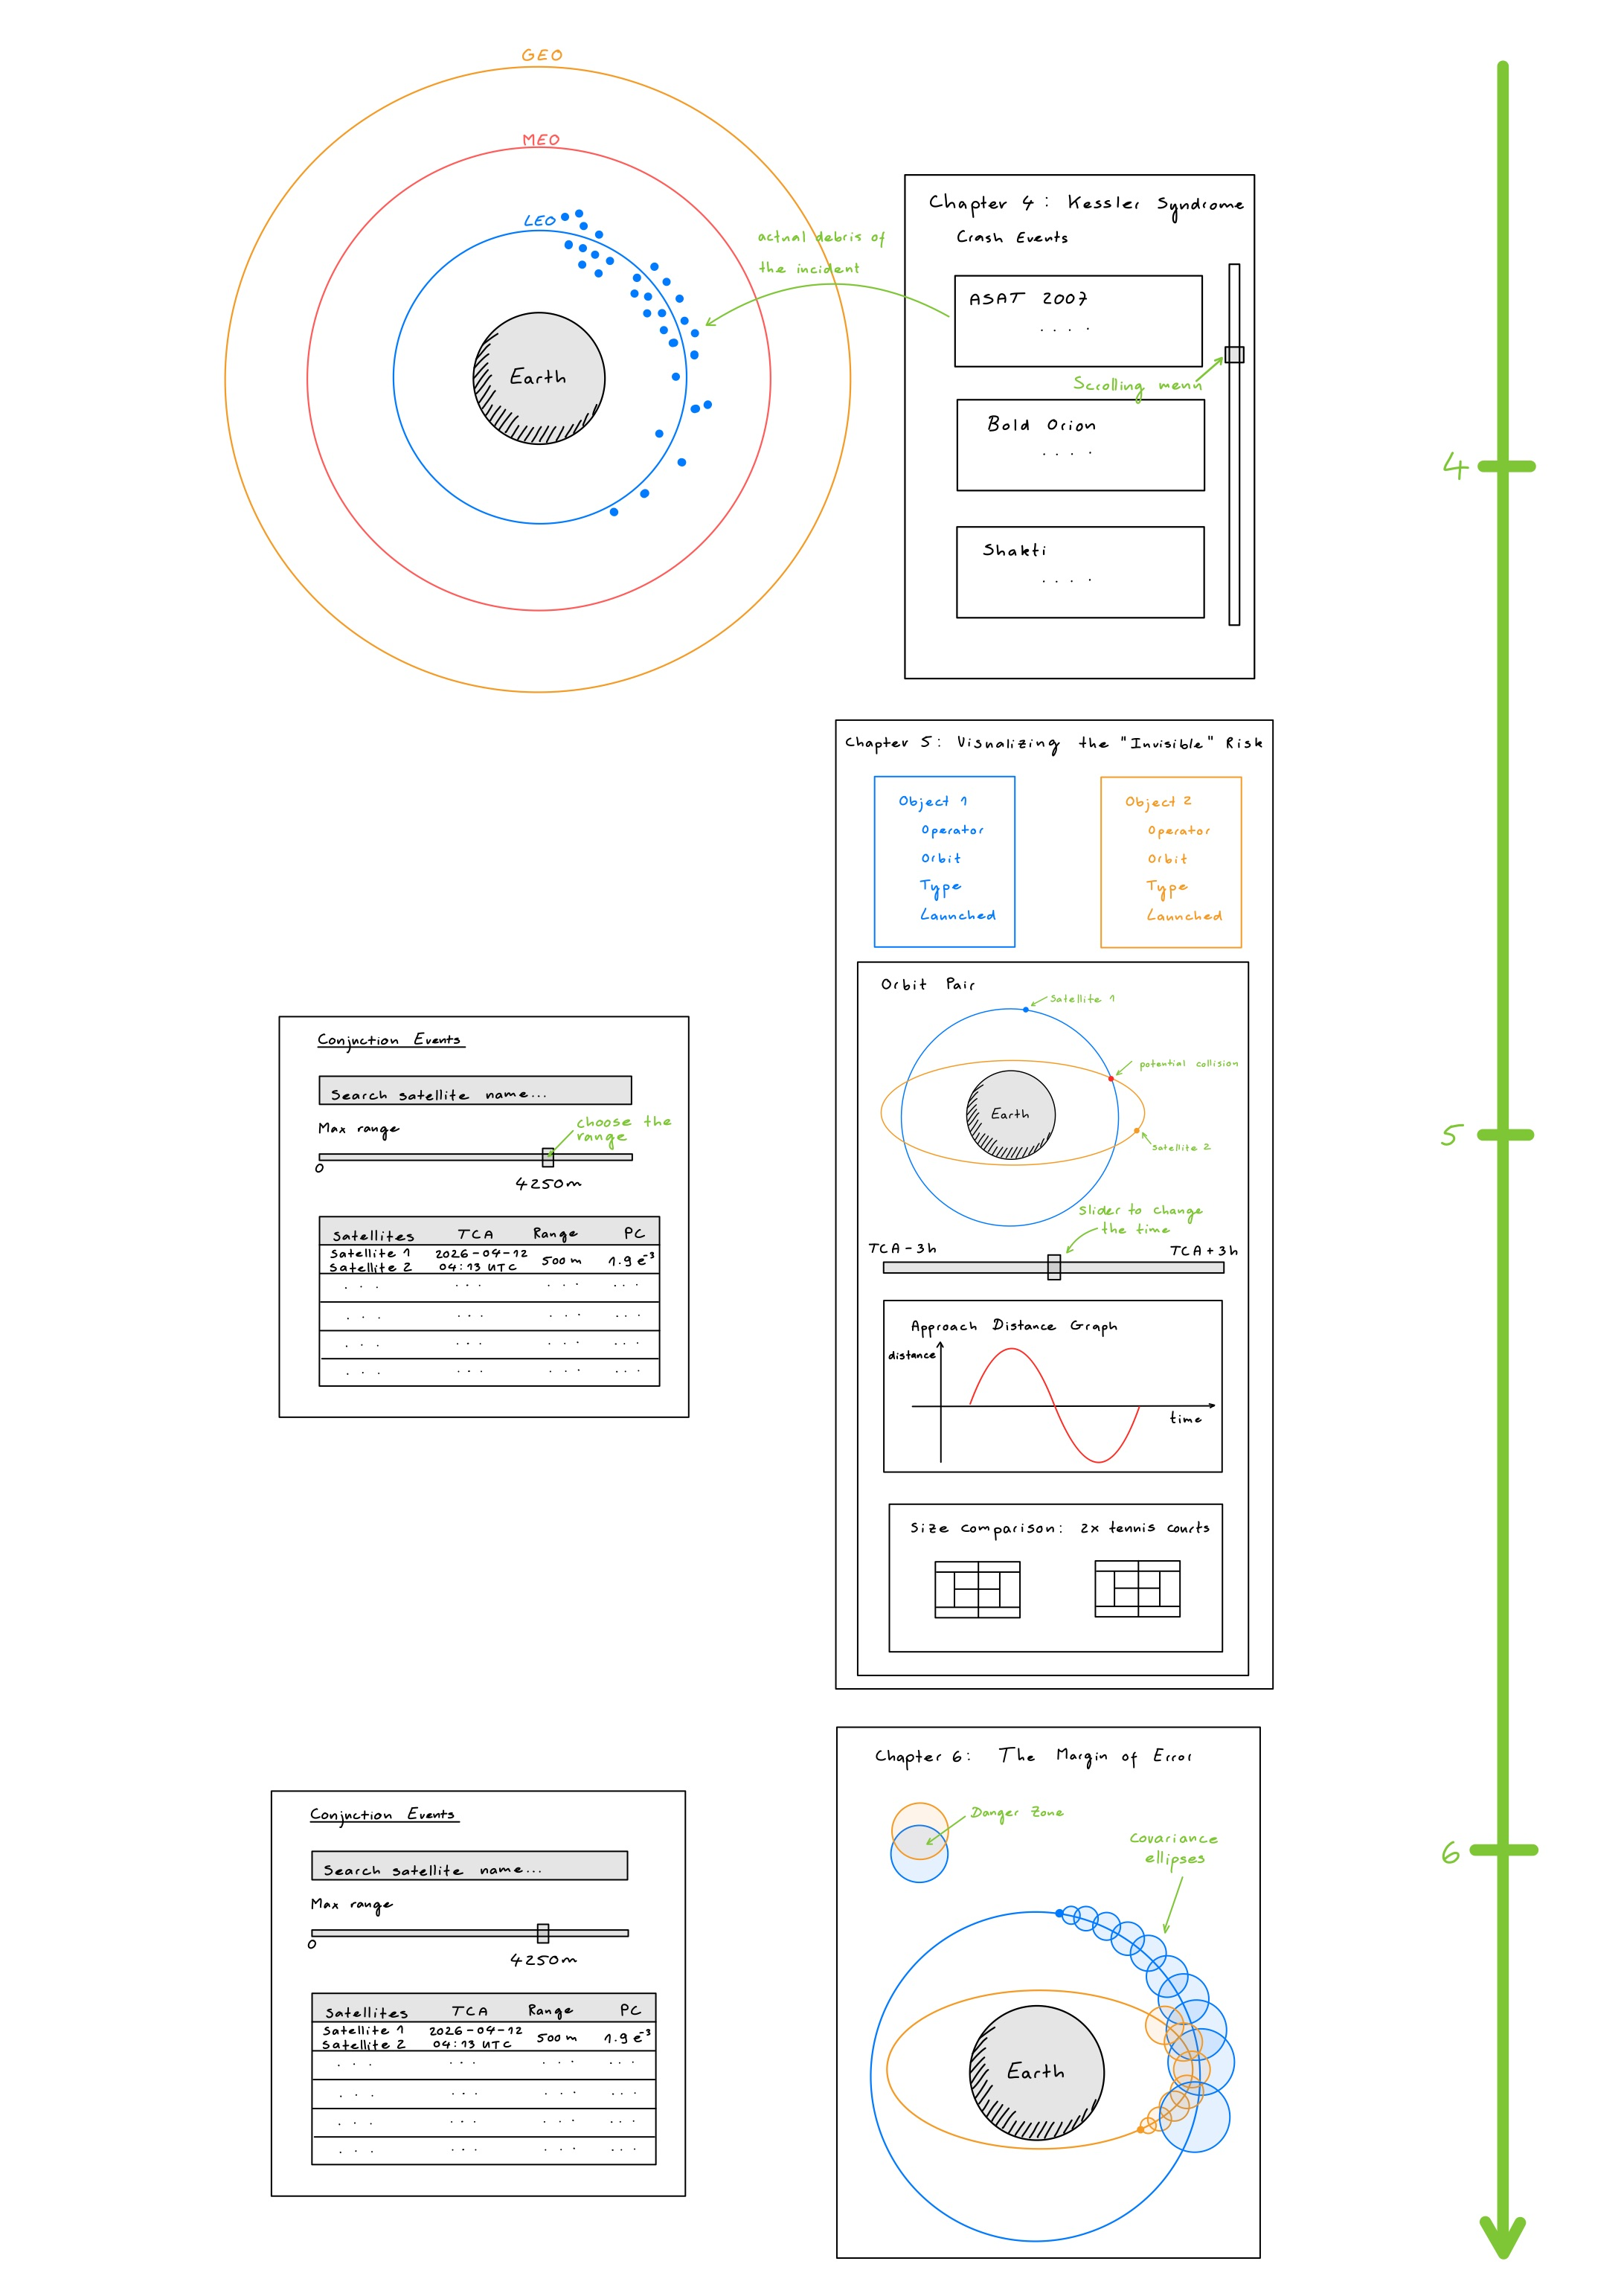
\includegraphics[width=1\linewidth]{Data Vizualization-9.jpg}
\end{figure}
